
En programmation il est très courant de vouloir conserver des données durant l'exécution du programme.
Nous parlerons ici uniquement des données qui sont dans la mémoire vive, c'est à dire la mémoire tampon 
de l'ordinateur, contrairement à la mémoire morte, qui est souvent un disque dur ou un CD.
Pour conserver une information dans la mémoire vive, il faut généralement créer une variable. Nous détaillerons 
ici tout ce que l'on peut faire avec des variables.

\section{Les Types}
\label{DefTypes}
Une machine étant une suite de transistors, et la mémoire vive une suite de cases vides et pleines :
tout est un nombre binaire. Mais les langages de programmation permettent de faire abstraction de cette complexité techinque.
Il existe donc en Vala différents types : 
\begin{itemize}
  \item int : entier, avec des variantes commes : « uint » (entier uniquement positif), ou « int32 » (grand entier)
  \item float : nombre à virgule 
  \item double : nombre à virgule à double précision
  \item char : caractère (en réalité c'est un entier positif de maximum 256, qui est traduit en caractères ensuite)
  \item string\footnote{String = chaîne, sous entendu chaîne de caractères} : tableau de char, donc du texte vu qu'un char est un caractère.
\end{itemize}

Ces types sont la base du langage, et on les retrouve souvent car c'est la forme la plus simple de conserver une donnée.
Mais il existe un autre type, légèrement plus complexe, qui permet de faire beaucoup plus de choses.

\section{Le pointeur}
Pour commencer il faut comprendre comment fonctionne la mémoire de notre ordinateur : 
\begin{figure}[H]
  \begin{center}
	  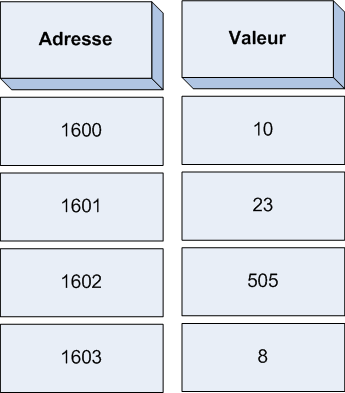
\includegraphics[width=12em]{Annexes/Images/tableau.png}
	\end{center}
	\caption{La mémoire}
\end{figure}

Ce code demande une case mémoire avec une adresse, et met le nombre 3 dedans.

\begin{lstlisting}
  int a = 3;
\end{lstlisting}

On peut récupérer l'adresse d'une variable. Par exemple pour afficher la valeur de a, puis son addresse en mémoire : 

\begin{lstlisting}
  printf ("La valeur est %d",a);
  printf ("L'adresse est %p",&a);
\end{lstlisting}

Le plus intéressant est qu'une adresse est un nombre, donc on peut la conserver dans une variable aussi !
La syntaxe est la suivante (avec type étant type du langage) : 

\begin{lstlisting}
  Type age = valeur;
  Type* pointeurSurAge = &age;
\end{lstlisting}

Ce qui donne en mémoire : 

\begin{figure}[H]
	\begin{center}
	  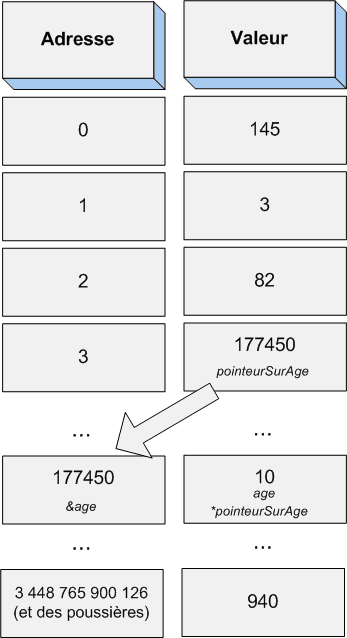
\includegraphics[width=12em]{Annexes/Images/pointeurs.png}
	\end{center}
	\caption{Un exemple de pointeur}
\end{figure}

On peut ensuite accéder à la valeur pointée par un pointeur avec la syntaxe suivante : 
\begin{lstlisting}
  *pointeurSurAge; // renvoie la valeur de age
\end{lstlisting}

Les pointeurs ne sont que des variables qui contiennent des adresses mémoire. Mais pour que l'ordinateur comprenne comment traiter la valeur pointée, le pointeur doit 
avoir le type de la variable (suivie de l'étoile du pointeur).

Une application directe du pointeur est le tableau.

\section{Tableaux}
\label{DefTableaux}
Un tableau est une suite de cases mémoire du même type : 
\begin{lstlisting}
  int tableau[4]; // Un tableau de 4 cases avec des int
  printf ("%d", tableau[1]); // valeur de la case 1
  tableau[10] = 2; // modifie une valeur du tableau
\end{lstlisting}

En réalité, voilà à quoi ressemble un tableau dans la mémoire de l'ordinateur\footnote{Image tirée de : \url{http://www.siteduzero.com/tutoriel-3-14015-les-tableaux.html}} : 
\begin{figure}[H]
	\begin{center}
	  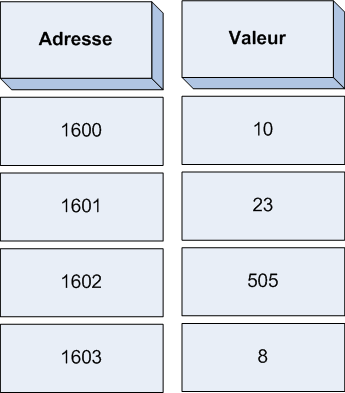
\includegraphics[width=12em]{Annexes/Images/tableau.png}
	\end{center}
	\caption{Un tableau dans la mémoire}
\end{figure}

Lorsqu'un tableau est créé, il prend un espace contigu en mémoire : les cases sont les unes à la suite des autres. L'ordinateur « saura » que c'est un tableau, et quand on demande la 3ème valeur, il prend la 3ème en partant de la première case du tableau. C'est pour cela qu'il peut y avoir les dépassements et bugs définits plus haut !

Donc en réalité, en Vala, un tableau est un pointeur vers la première variable d'une suite de variables contigues. On peut donc considérer que : 
\begin{lstlisting}
  *(tableau); // envoie la valeur de la case d'adresse 'tableau'
  tableau[0]; // envoie la case 0
  *(tableau + 3); //  envoie la valeur de la cases d'adresse 'tableau' + 3
  tableau[3]; // envoie la case 3 ( quatrieme car on compte de 0 )
\end{lstlisting}
Les syntaxes sont différentes, mais mènent au même résultat, et expliquent un peu mieux le fonctionnement du tableau.

Il en découle que le tableau a une taille fixe. Et que pour l'agrandir, il faut trouver un espace suffisant de cases mémoire contigues.

\begin{quotation}
  Le langage C n'impose pas à une implémentation de vérifier les accès, en écriture comme en lecture, hors des limites d'un tableau ; il précise explicitement qu'un tel code a un comportement indéfini, donc que n'importe quoi peut se passer. En l'occurence, ce code peut très bien marcher comme on pourrait l'attendre […] ou causer un arrêt du programme avec erreur […] ou encore corrompre une autre partie de la mémoire du processus […] ce qui peut modifier son comportement ultérieur de manière très difficile à prévoir.
  \begin{flushright}
    Wikipédia
  \end{flushright}
\end{quotation}

Il faut donc faire très attention à ne jamais dépasser la taille d'un tableau !


\section{Ennumération}
L'énnumération permet de créer un nouveau type qui peut prendre 
un certain nombre de valeurs dans un ensemble fini, imaginons un type « Volume » 
qui peut avoir uniquement les valeurs suivantes : FORT, MOYEN, FAIBLE, NULL, INFINI : 

\begin{lstlisting} 
  enum Volume {
    FORT, FAIBLE, MOYEN, NULL, INFINI
  };
  
  Volume a = Volume.FORT;
\end{lstlisting}

Ceci est utilisé pour clarifier le code, il est toujours plus lisible de faire des conditions avec des mots, plutôt qu'avec des nombres.
Par exemple, le menu a un certain nombre d'actions, au lieu de leur associer un nombre, on leur associe une valeur de l'énumération « ActionMenu ».

Mais si ceci permet quasi-uniquement de clarifier le code, il existe un moyen de créer nos propres types plus complexes.

\section{Structures}
\label{DefStruct}
Une structure est un type qui permet de combiner des variables : 
\begin{lstlisting}
  typedef struct Personne {
    int age;
    string nom;
  };
  
  Personne p;
  p.age = 16;
  p.nom = "jaques";
\end{lstlisting}

C'est à partir de cette structure que l'on peut définir des structures plus complexes.

\section{Listes}
\label{DefListe}
Les listes sont des structures plus complexes, et qui ne sont malheureusement pas gérées directement par le C ( mais par le Vala oui ).
On fait en réalité la chose suivante : 
\begin{figure}[H]
	\begin{center}
	  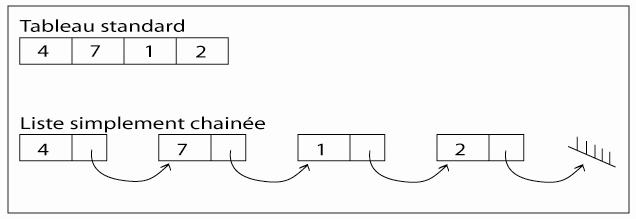
\includegraphics[width=20em]{Annexes/Images/liste.jpg}
	\end{center}
	\caption{Une liste chainée et un tableau}
\end{figure}
\begin{lstlisting}
  struct element
  {
      int val;
      element *nxt; // pointeur vers l'element suivant
  };
\end{lstlisting}

On a donc uniquement des structures qui se pointent les unes vers les autres, sans avoir besoin de zones contigues. Les opérations d'ajout et de suppression d'élément sont plus rapides : 
\begin{figure}[H]
	\begin{center}
	  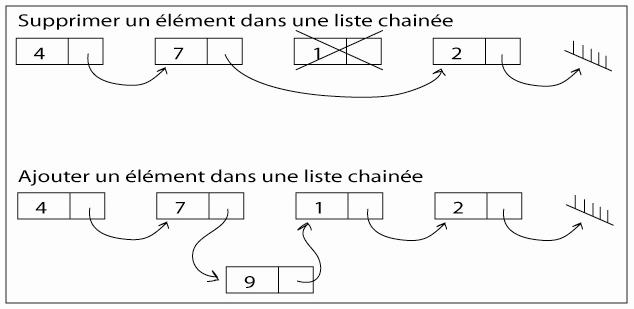
\includegraphics[width=20em]{Annexes/Images/liste_ajout.jpg}
	\end{center}
	\caption{Ajout et suppression d'un item à la liste}
\end{figure}

Mais pour récupérer un élément, on est obligé de parcourir la liste. Ce qui fait perdre du temps. Pour récupérer l'élément 3, il faut aller au un, puis au deux, et enfin regarder la valeur du numéro 3 !
Ce qui est bien moins efficace qu'un tableau. Il n'y a donc pas que des avantages, ni que des inconvénients. Les listes ne sont pas toujours simplement chainées, on peut aussi en avoir des doublement chainées, c'est à dire que chaque élément pointe vers le suivant ET le précédent. Il peut aussi y avoir des listes cycliques, c'est à dire que le dernier élément pointe vers le premier.
